\documentclass[platex,dvipdfmx]{jsarticle}
\usepackage{color}
\usepackage{listings,jvlisting}
\usepackage[dvipdfmx]{graphicx}
\usepackage{here}
\lstset{
  language=Python,
  basicstyle={\ttfamily},
  identifierstyle={\small},
  commentstyle={\small\itshape},
  keywordstyle={\small\bfseries\color{red}},
  ndkeywordstyle={\small},
  stringstyle={\small\ttfamily\color{yellow}},
  frame={tb},
  breaklines=true,
  columns=[l]{fullflexible},
  numbers=left,
  xrightmargin=0zw,
  xleftmargin=3zw,
  numberstyle={\scriptsize},
  stepnumber=1,
  numbersep=1zw,
  lineskip=-0.5ex
}
\renewcommand{\lstlistingname}{ソースコード}
\begin{document}
\title{課題4レポート}
\author{羽路 悠斗}
\maketitle

\section{課題内容}

MNISTのテスト画像1枚を入力とし、3層ニューラルネットワークを用いて、0~9の値のうち1つを出力するプログラムを作成せよ。

\section{作成したプログラムの説明}

\subsection{ディレクトリ構造}

モデルの構造やパラメータを変えて実験したかったので、ディレクトリを以下のように構造化する。historyディレクトリには、訓練ごとに全エポックのlossとaccが格納されている。modelディレクトリには、訓練ごとに最適なエポックの重みが格納されている。logディレクトリにはログが格納されている。

\noindent
ex4\_im \\
\textbar --contest.py \\
\textbar --ex\_advanced.py \\
\textbar --history \\
\textbar \, \textbar --0000\_history.dump \\
\textbar --log \\
\textbar \, \textbar --general.log \\
\textbar --logger.py \\
\textbar --model \\
\textbar \, \textbar --0000.npz \\

\subsection{設計方針}

オプティマイザ、レイヤ、モデルをそれぞれクラス化する。これによりプログラムの可読性が上がり、拡張性や可変性も上がる。特にコンテストにおいては、実験を繰り返す必要があるので、以上の性能は重要である。

また基本的に$(batch\_size, height, width)$のndarrayでデータを保持する。平坦化した際も、先頭の次元がbatch\_sizeを表す。なお、畳み込みそうなどでチャンネルを表す次元が必要になるときは$(batch\_size, channel, height, width)$を使う。

\subsection{各層の説明}

\subsubsection{ベース}

まずは層のベースとなるLayerクラスをソースコード\ref{Layer}に示す。全てのレイヤはLayerクラスのサブクラスとして実装する。クラス内の各関数について簡単に説明する。

\begin{itemize}
  \item コンストラクタは、層の重みとオプティマイザを初期化する。
  \item forward関数は前の層の出力を受け取り、この層の出力を返す。逆伝搬処理で使うことがあるので、入出力をクラス変数として保持しておく。学習時と推論時で異なる動作をする層があるので、フラグも受け取る。
  \item backward関数は次の層の勾配を受け取り、この層の勾配を返す。重みの更新で使うことがあるので、勾配をクラス変数として保持しておく。
  \item update関数はオプティマイザに重みの香辛料を計算させ更新する。
  \item get\_weight関数はこの層の重みを表す辞書を返す。
  \item load\_weight関数は全ての層の重みを表す辞書を受け取り、自身に当てはまる重みをロードする。
\end{itemize}

\begin{lstlisting}[caption=ex\_advanced.py, label=Layer]
class Layer:
  def __init__(self, *args, **kwds):
    pass

  def forward(self, x, *args, **kwds):
    self.x = x
    self.y = x
    return self.y

  def backward(self, grad, *args, **kwds):
    self.grad_x = grad
    return self.grad_x

  def update(self, *args, **kwds):
    pass

  def get_weight(self, *args, **kwds) -> tuple:
    return {}

  def load_weight(self, weight_dic):
    pass
\end{lstlisting}

\newpage

\subsubsection{入力層}

入力層はMNIST画像を指定された形状に変形する。すなわち、1次元化するか2次元のまま扱うかである。

\begin{itemize}
  \item コンストラクタには、データの形を指定する。
  \item forward関数で、画像データを指定された形に変形する。
\end{itemize}

\begin{lstlisting}[caption=ex\_advanced.py, label=Input]
class Input(Layer):
  def __init__(self, output_shape: tuple):
    self.output_shape = output_shape
    self.output_dim = len(output_shape)
  
  def forward(self, x, batch_size=100, mode='train'):
    self.x = x
    if self.output_dim == 1:  # 1次元化
      self.y = x.reshape((batch_size,) + self.output_shape).T
    else:  # 画像データをそのまま扱う場合を想定
      self.y = x.reshape((batch_size,) + self.output_shape)
\end{lstlisting}

\subsubsection{全結合層}

全結合層の出力は、重みベクトルを$W$、バイアスベクトルを$B$とおくと、次のように計算される。

\[
  WX + B
\]

逆伝搬は、クロスエントロピー誤差の平均を$E_n$として、次のように計算される。

\[
  \frac{\delta E_n}{\delta X} = W^T \frac{\delta E_n}{\delta Y} \\
  \frac{\delta E_n}{\delta W} = \frac{\delta E_n}{\delta Y} X^T \\
  \frac{\delta E_n}{\delta B} = rowSum(\frac{\delta E_n}{\delta Y})
\]

\begin{itemize}
  \item コンストラクタには中間層のノード数、入力サイズ、層の名前、オプティマイザとその引数を指定し、それらと重みを初期化する。
  \item forward関数で、numpyの行列積を用いて出力を計算する。
  \item backward関数で、勾配を計算する。こちらもnumpyの行列積を用いる。
\end{itemize}

\begin{lstlisting}[caption=ex\_advanced.py, label=Dense]
class Dense(Layer):
  def __init__(self, units: int, input_size: int, name: str='dense', opt: str='SGD', opt_kwds: dict={}):
    self.units = units

    self.w = random.normal(loc=0, scale=np.sqrt(1/input_size), size=input_size*units).reshape(units, input_size)
    self.b = random.normal(loc=0, scale=np.sqrt(1/input_size), size=units)
    self.name = name
    self.opt = get_opt(opt, **opt_kwds)

  def forward(self, x, batch_size=100, mode='train'):
    self.x = x
    self.batch_size = batch_size
    self.y = self.w@self.x + self.b.reshape(-1, 1)
    return self.y

  def backward(self, grad):
    self.grad_x = self.w.T@grad
    self.grad_w = grad@self.x.T
    self.grad_b = np.sum(grad, axis=1)
    return self.grad_x

  def update(self):
    dw, db = self.opt.update(self.grad_w, self.grad_b)
    self.w += dw
    self.b += db

  def get_weight(self) -> tuple:
    return {f'{self.name}_w': self.w, f'{self.name}_b': self.b}

  def load_weight(self, weight_dic):
    self.w = weight_dic[f'{self.name}_w']
    self.b = weight_dic[f'{self.name}_b']
\end{lstlisting}

\newpage

\subsubsection{畳み込み層}

畳み込み層によって画像を2次元のまま扱えるので、精度向上が見込める。なおim2colとcol2imを用いて画像と行列を変換することで処理を高速化できるが、ここでは詳細は省く。

順伝搬は、im2colで処理した入力を用いると簡単に計算できる。

\[
  WX + B
\]

逆伝搬も、im2colで処理した入力を用いると簡単に計算できる。

\[
  \frac{\delta E_n}{\delta X} = W^T \frac{\delta E_n}{\delta Y} \\
  \frac{\delta E_n}{\delta W} = \frac{\delta E_n}{\delta Y} X^T \\
  \frac{\delta E_n}{\delta B} = rowSum(\frac{\delta E_n}{\delta Y})
\]

ただし入力の勾配は、col2imを通してから逆伝搬させることに注意。

\begin{itemize}
  \item コンストラクタには、入力の形、フィルタの形、フィルタの枚数、層の名前、オプティマイザとその引数を指定し、初期化する。
  \item さらに、フィルタの重みとバイアスを初期化する。その他、再利用する数は計算しておく。
  \item フィルタはあらかじめ行列で表しておく。
  \item im2colは画像を受け取り、便利な形の行列に変換する内部関数である。
  \item col2imはim2colの逆の動作をする。
  \item forward関数で、im2col、畳み込み演算、形を標準に戻す、の順に処理する。
  \item backward関数で、次の層の勾配をフィルタと対応する形の行列に変形、この層の勾配を計算、の順に処理する。
\end{itemize}

\begin{lstlisting}[caption=ex\_advanced.py, label=Conv]
class Conv(Layer):
  def __init__(self, *, input_shape: tuple, filter_shape: tuple, filter_num: int, name: str='conv', opt: str='SGD', opt_kwds: dict={}):
    self.im_h = input_shape[0]
    self.im_w = input_shape[1]
    self.filter_h = filter_shape[0]
    self.filter_w = filter_shape[1]
    self.pad_h = math.floor(self.filter_h/2)
    self.pad_w = math.floor(self.filter_w/2)
    self.o_h = self.im_h-self.filter_h+2*self.pad_h+1
    self.o_w = self.im_w-self.filter_w+2*self.pad_w+1
    self.filter_num = filter_num
    self.w = 0.05*random.randn(self.filter_num, self.filter_h*self.filter_w)
    self.b = 0.05*random.randn(self.filter_num)
    self.name = name
    self.opt = get_opt(opt, **opt_kwds)

  def _im2col(self, im, batch_size):
    pad_wid = ((0, 0), (self.pad_h, self.pad_h), (self.pad_w, self.pad_w))
    pad_im = np.pad(im, pad_wid)
    col = np.empty((batch_size, self.filter_h, self.filter_w, self.o_h, self.o_w))  # (batch size, filter height, filter width, output height, output width)
    for h in range(self.filter_h):
      for w in range(self.filter_w):
        col[:, h, w, :, :] = pad_im[:, h : h+self.o_h, w : w+self.o_w]
    col = col.transpose(1, 2, 0, 3, 4).reshape(self.filter_w*self.filter_h, batch_size*self.o_w*self.o_h)
    return col

  def _col2im(self, col, batch_size):
    col = col.reshape(self.filter_h, self.filter_w, batch_size, self.o_h, self.o_w).transpose(2, 0, 1, 3, 4)
    im = np.zeros((batch_size, self.im_h+2*self.pad_h, self.im_w+2*self.pad_w))
    for h in range(self.filter_h):
      for w in range(self.filter_w):
        im[:, h : h+self.o_h, w : w+self.o_w] += col[:, h, w, :, :]
    return im

  def forward(self, x, batch_size=100, mode='train'):
    self.x = self._im2col(x, batch_size)
    self.batch_size = batch_size
    self.y = self.w@self.x + self.b.reshape(-1, 1)
    self.y = self.y.reshape(self.filter_num, batch_size, self.o_h, self.o_w).transpose(1, 0, 2, 3)
    return self.y

  def backward(self, grad):
    grad = grad.transpose(1, 0, 2, 3).reshape(self.filter_num, self.batch_size*self.o_h*self.o_w)
    self.grad_x = self._col2im(self.w.T@grad, self.batch_size)
    self.grad_w = grad@self.x.T
    self.grad_b = np.sum(grad, axis=1)
    return self.grad_x

  def update(self):
    dw, db = self.opt.update(self.grad_w, self.grad_b)
    self.w += dw
    self.b += db

  def get_weight(self) -> tuple:
    return {f'{self.name}_w': self.w, f'{self.name}_b': self.b}

  def load_weight(self, weight_dic):
    self.w = weight_dic[f'{self.name}_w']
    self.b = weight_dic[f'{self.name}_b']
\end{lstlisting}

\newpage

\subsubsection{プーリング}

プーリング層は畳み込み層で捉えられた特徴を「ぼかす」働きがある。具体的には2*2maxプーリングだと2*2の領域で最大のものを出力にする。これも処理を高速化するためにim2colとcol2imを用いる。畳み込みそうで用いられるものとは行列の形が少し異なる。

逆伝搬は、順伝搬時にプーリングで抽出されたインデックスに勾配を当てはめて、その他の勾配は0として伝搬する。

\begin{itemize}
  \item コンストラクタには、入力の形とチャンネル数とプーリング層のサイズを指定する。
  \item forward関数で、im2col、プーリングを順に処理する。逆伝播のために、プーリングで抽出されたインデックスを保持しておく。
  \item backward関数で、勾配を行列で表してから、col2imを通す。
\end{itemize}

\begin{lstlisting}[caption=ex\_advanced.py, label=Pooling]
class Pooling(Layer):
  def __init__(self, *, input_shape: tuple, channel: int, pool_shape: tuple):
    self.im_h = input_shape[0]
    self.im_w = input_shape[1]
    self.channel = channel
    self.pool_h = pool_shape[0]
    self.pool_w = pool_shape[1]
    self.o_h = self.im_h//self.pool_h
    self.o_w = self.im_w//self.pool_w

  def _im2col(self, im, batch_size):
    col = np.empty((batch_size, self.channel, self.pool_h, self.pool_w, self.o_h, self.o_w))
    for h in range(self.pool_h):
      for w in range(self.pool_w):
        col[:, :, h, w, :, :] = im[:, :, h : h+self.pool_h*self.o_h : self.pool_h, w : w+self.pool_w*self.o_w : self.pool_w]
    col = col.transpose(0, 1, 4, 5, 2, 3).reshape(batch_size*self.channel*self.o_h*self.o_w, self.pool_h*self.pool_w)
    return col

  def _col2im(self, col, batch_size):
    col = col.reshape(self.batch_size, self.channel, self.o_h, self.o_w, self.pool_h, self.pool_w).transpose(0, 1, 4, 5, 2, 3)
    im = np.zeros((batch_size, self.channel, self.im_h, self.im_w))
    for h in range(self.pool_h):
      for w in range(self.pool_w):
        im[:, :, h : h+self.pool_h*self.o_h : self.pool_h, w : w+self.pool_w*self.o_w : self.pool_w] += col[:, :, h, w, :, :]
    return im

  def forward(self, x, batch_size=100, mode='train'):
    self.x = self._im2col(x, batch_size)
    self.batch_size = batch_size
    self.ind = np.argmax(self.x, axis=1)
    self.y = np.max(self.x, axis=1).reshape((batch_size, self.channel, self.o_h, self.o_w))
    return self.y

  def backward(self, grad):
    self.grad_x = np.zeros((self.batch_size*self.channel*self.o_h*self.o_w, self.pool_h*self.pool_w))
    self.grad_x[np.arange(self.ind.size), self.ind] = grad.flatten()
    self.grad_x = self._col2im(self.grad_x, self.batch_size)
    return self.grad_x
\end{lstlisting}

\subsubsection{平坦化層}

Flatten層は、画像を全結合層の入力にできるように平坦化する。順伝搬は、バッチ次元はそのままで、他の次元を平坦化する。逆伝搬は、順伝播と逆の変形をする。

\begin{lstlisting}[caption=ex\_advanced.py, label=Flatten]
class Flatten(Layer):
  def __init__(self):
    pass

  def forward(self, x, batch_size=100, mode='train'):
    self.x = x
    self.batch_size = batch_size
    self.y = x.reshape((batch_size, -1)).T
    return self.y
  
  def backward(self, grad):
    self.grad_x = grad.T.reshape((self.batch_size, *self.x.shape[1:]))
    return self.grad_x
\end{lstlisting}

\newpage

\subsubsection{シグモイド}

シグモイド関数は、活性化関数の一種で、値を0〜1の範囲に変換する。順伝搬は次の式で表せる。なお、シグモイド関数はこの式からわかるように、絶対値の大きな数を扱うことが苦手である。そのため、後述する正規化が望ましい。

\[
  \frac{1}{1 + exp(-x)}
\]

逆伝搬は次の式で表せる。

\[
  \frac{\delta E_n}{\delta x} = \frac{\delta E_N}{\delta y}(1-y)y
\]

\begin{itemize}
  \item forward関数で、オーバーフローに対処するために閾値を超えた値を丸める。
\end{itemize}

\begin{lstlisting}[caption=ex.advanced.py, label=Sigmoid]
class Sigmoid(Layer):
  def __init__(self):
    pass

  def forward(self, x, batch_size=100, mode='train'):
    sigmoid_range = 34.538776394910684
    x = np.clip(x, -sigmoid_range, sigmoid_range)
    self.x = x
    self.y = 1/(1.0+np.exp(-x))
    return self.y

  def backward(self, grad):
    self.grad_x = grad*(1-self.y)*self.y
    return self.grad_x
\end{lstlisting}

\subsubsection{ReLU}

ReLU関数は、活性化関数の1種で、0以下の値を0に丸める。負の値をノイズと見做していると考えることができ、画像は値が正なので相性がいいとされる。

\[
  a(t) = \left\{ \begin{array}{l}
  t ( t > 0 ) \\
  0 ( t \leq 0 )
  \end{array} \right.
\]

勾配は次の通り。

\[
  a(t)' = \left\{ \begin{array}{l}
  1 ( t > 0 ) \\
  0 ( t \leq 0 )
  \end{array} \right.
\]

\begin{lstlisting}[caption=ex\_advanced.py, label=ReLU]
class ReLU(Layer):
  def __init__(self):
    pass

  def forward(self, x, batch_size=100, mode='train'):
    self.x = x
    self.y = np.where(x>0, x, 0)
    return self.y

  def backward(self, grad):
    self.grad_x = grad*np.where(self.x>0, 1, 0)
    return self.grad_x
\end{lstlisting}

\subsubsection{バッチノーマリゼーション}

バッチノーマリゼーションは、各ノードのミニバッチの出力が分散1、平均0となるように正規化する処理である。順伝播と逆伝播の式の記述は、講義資料に任せる。コードの量は多いが、実装に難しい点はなく、式を愚直にプログラムに変換するのみである。1点、numpyでsumをとると次元が小さくなるので、大きさ1の次元をnp.expand\_dims()で補完することに注意。

\begin{lstlisting}[caption=ex\_advanced.py, label=BatchNormalization]
class BatchNormalization(Layer):
  def __init__(self, units: int=96, name: str='bn', opt: str='SGD', opt_kwds: dict={}):
    self.name = name
    self.opt = get_opt(opt, **opt_kwds)
    self.gamma = np.ones((units,1))
    self.beta = np.zeros((units,1))
    self.mean_list = []
    self.variance_list = []

  def forward(self, x, batch_size=100, mode='train'):
    if mode == 'train':
      self.x = x
      self.batch_size = batch_size
      self.mean = np.expand_dims(np.sum(x, axis=1)/self.batch_size, axis=-1)
      self.variance = np.expand_dims(np.sum(np.square(x-self.mean), axis=1)/self.batch_size, axis=-1)
      self.x_normalized = (x-self.mean)/np.sqrt(self.variance+sys.float_info.epsilon)
      self.y = self.gamma*self.x_normalized + self.beta
      self.mean_list.append(self.mean)
      self.variance_list.append(self.variance)
      self.mean_expected = np.average(np.array(self.mean_list), axis=0)
      self.variance_expected = np.average(np.array(self.variance_list), axis=0)
      return self.y
    elif mode == 'inference':
      return self.gamma/np.sqrt(self.variance_expected+sys.float_info.epsilon)*x + (self.beta - self.gamma*self.mean_expected/np.sqrt(self.variance_expected+sys.float_info.epsilon))
    else:
      raise ValueError('mode is train or inference.')

  def backward(self, grad):
    self.grad_x_normalized = grad*self.gamma
    self.grad_variance = np.expand_dims(np.sum(grad*(self.x-self.mean)*(-1)/2*np.power(self.variance+sys.float_info.epsilon, -3/2), axis=1), axis=-1)
    self.grad_mean = np.expand_dims(np.sum(self.grad_x_normalized*(-1)/np.sqrt(self.variance+sys.float_info.epsilon), axis=1), axis=-1) + self.grad_variance*np.expand_dims(np.sum(-2*(self.x-self.mean), axis=1)/self.batch_size, axis=-1)
    self.grad_x = self.grad_x_normalized/np.sqrt(self.variance+sys.float_info.epsilon) + self.grad_variance*2*(self.x-self.mean)/self.batch_size + self.grad_mean/self.batch_size
    self.grad_gamma = np.expand_dims(np.sum(grad*self.x_normalized, axis=1), axis=-1)
    self.grad_beta = np.expand_dims(np.sum(grad, axis=1), axis=-1)
    return self.grad_x

  def update(self):
    dgamma, dbeta = self.opt.update(self.grad_gamma, self.grad_beta)
    self.gamma += dgamma
    self.beta += dbeta

  def get_weight(self) -> tuple:
    return {f'{self.name}_gamma': self.gamma, f'{self.name}_beta': self.beta}

  def load_weight(self, weight_dic):
    self.gamma = weight_dic[f'{self.name}_gamma']
    self.beta = weight_dic[f'{self.name}_beta']
\end{lstlisting}

\subsubsection{ドロップアウト}

ドロップアウトは、層のノードをランダムに無視する手法である。過学習の抑制に効果的だとされる。

\begin{itemize}
  \item forward関数で、フラグによって学習時と推論時で動作を変えている。
\end{itemize}

\[
  a(t) = \left\{ \begin{array}{l}
  t ( 無視されない場合 ) \\
  0 ( 無視される場合 )
  \end{array} \right.
\]

勾配は次の通り。

\[
  a(t)' = \left\{ \begin{array}{l}
  1 ( 無視されない場合 ) \\
  0 ( 無視される場合 )
  \end{array} \right.
\]

\begin{lstlisting}[caption=ex\_advanced.py, label=Dropout]
class Dropout(Layer):
  def __init__(self, dropout: float=0.1):
    self.dropout = dropout
  
  def forward(self, x, batch_size=100, mode='train'):
    self.x = x
    if mode == 'train':
      self.mask = (np.random.rand(*self.x.shape) >= self.dropout)
      self.y = x*self.mask
      return self.y
    elif mode == 'inference':
      return x*(1-self.dropout)
    else:
      raise ValueError('mode is train or inference.')

  def backward(self, grad):
    self.grad_x = grad*self.mask
    return self.grad_x
\end{lstlisting}

\subsubsection{ソフトマックス}
ソフトマックス関数は多クラス分類で出力層の活性化関数に用いられる。各クラスに属する尤度を表す。$\alpha$はオーバーフローを防ぐために導入する。

\[
  y_i = \frac{exp(x_i - \alpha)}{\Sigma_{j=1}^C exp(a_j - \alpha)}
\]

\[
  \alpha = max \, a_i
\]

逆伝搬は次の式で表せる。

\[
  \frac{\delta E_n}{\delta x_i} = \frac{y_i - y\_true_i}{batch\_size}
\]

\begin{lstlisting}[caption=ex\_advanced.py, label=Softmax]
class Softmax(Layer):
  def __init__(self):
    pass

  def forward(self, x, batch_size=100, mode='train'):
    self.batch_size = batch_size
    self.x = x
    self.y = np.exp(x-np.max(x, axis=0)) / (np.sum(np.exp(x-np.max(x, axis=0)), axis=0))
    return self.y

  def backward(self, true_y):
    grad_x = (self.y - true_y.T)/self.batch_size
    return grad_x
\end{lstlisting}

\newpage

\subsection{最適化}

オプティマイザは、実装が単純なので、ベースクラスは作成していない。コンストラクタで、学習率などのパラメータを初期化する。update関数で、重みとバイアスの勾配を受け取って、更新量を返す。それぞれの特性や式は、講義資料に説明があるので省略する。

\subsubsection{SGD}

\begin{lstlisting}[caption=ex\_advanced.py, label=SGD]
class SGD:
  def __init__(self, lr: float=0.01):
    self.lr = lr
  
  def update(self, grad_w, grad_b):
    dw = -self.lr*grad_w
    db = -self.lr*grad_b
    return dw, db
\end{lstlisting}

\subsubsection{慣性項付きSGD}

\begin{lstlisting}[caption=ex\_advanced.py, label=MomentumSGD]
class MomentumSGD:
  def __init__(self, lr: float=0.01, alpha: float=0.9):
    self.lr = lr
    self.alpha = alpha

  def update(self, grad_w, grad_b):
    self.dw = self.alpha*self.dw - self.lr*grad_w
    self.db = self.alpha*self.db - self.lr*grad_b
    return self.dw, self.db
\end{lstlisting}

\subsubsection{AdaGrad}

\begin{lstlisting}[caption=ex\_advanced.py, label=AdaGrad]
class AdaGrad:
  def __init__(self, lr: float=0.001, h0: float=1e-8):
    self.lr = lr
    self.h_w = h0
    self.h_b = h0

  def update(self, grad_w, grad_b):
    self.h_w = self.h_w + grad_w*grad_w
    self.h_b = self.h_b + grad_b*grad_b
    dw = -self.lr/np.sqrt(self.h_w)*grad_w
    db = -self.lr/np.sqrt(self.h_b)*grad_b
    return dw, db
\end{lstlisting}

\subsubsection{RMSProp}

\begin{lstlisting}[caption=ex\_advanced.py, label=RMSProp]
class RMSProp:
  def __init__(self, lr: float=0.001, rho: float=0.9, epsilon: float=1e-8, h0: float=1e-8):
    self.lr = lr
    self.rho = rho
    self.epsilon = epsilon
    self.h_w = h0
    self.h_b = h0

  def update(self, grad_w, grad_b):
    self.h_w = self.rho*self.h_w + (1-self.rho)*grad_w*grad_w
    self.h_b = self.rho*self.h_b + (1-self.rho)*grad_b*grad_b
    dw = -self.lr/np.sqrt(self.h_w)*grad_w
    db = -self.lr/np.sqrt(self.h_b)*grad_b
    return dw, db
\end{lstlisting}

\subsubsection{AdaDelta}

\begin{lstlisting}[caption=ex\_advanced.py, label=AdaDelta]
class AdaDelta:
  def __init__(self, rho: float=0.95, epsilon: float=1e-6):
    self.rho = rho
    self.epsilon = epsilon
    self.h_w = 0
    self.h_b = 0
    self.s_w = 0
    self.s_b = 0

  def update(self, grad_w, grad_b):
    self.h_w = self.rho*self.h_w + (1-self.rho)*grad_w*grad_w
    self.h_b = self.rho*self.h_b + (1-self.rho)*grad_b*grad_b
    dw = -np.sqrt(self.s_w+self.epsilon)/np.sqrt(self.h_w+self.epsilon)*grad_w
    db = -np.sqrt(self.s_b+self.epsilon)/np.sqrt(self.h_b+self.epsilon)*grad_b
    self.s_w = self.rho*self.s_w + (1-self.rho)*dw*dw
    self.s_b = self.rho*self.s_b + (1-self.rho)*db*db
    return dw, db
\end{lstlisting}

\subsubsection{Adam}

\begin{lstlisting}[caption=ex\_advanced.py, label=Adam]
class Adam:
  def __init__(self, alpha: float=0.001, beta_1: float=0.9, beta_2: float=0.999, epsilon: float=1e-8):
    self.alpha = alpha
    self.beta_1 = beta_1
    self.beta_2 = beta_2
    self.epsilon = epsilon
    self.t = 0
    self.m_w = 0
    self.m_b = 0
    self.v_w = 0
    self.v_b = 0

  def update(self, grad_w, grad_b):
    self.t = self.t+1
    self.m_w = self.beta_1*self.m_w + (1-self.beta_1)*grad_w
    self.m_b = self.beta_1*self.m_b + (1-self.beta_1)*grad_b
    self.v_w = self.beta_2*self.v_w + (1-self.beta_2)*grad_w*grad_w
    self.v_b = self.beta_2*self.v_b + (1-self.beta_2)*grad_b*grad_b
    self.m_w_hat = self.m_w/(1-np.power(self.beta_1, self.t))
    self.m_b_hat = self.m_b/(1-np.power(self.beta_1, self.t))
    self.v_w_hat = self.v_w/(1-np.power(self.beta_2, self.t))
    self.v_b_hat = self.v_b/(1-np.power(self.beta_2, self.t))
    dw = -self.alpha*self.m_w_hat/(np.sqrt(self.v_w_hat)+self.epsilon)
    db = -self.alpha*self.m_b_hat/(np.sqrt(self.v_b_hat)+self.epsilon)
    return dw, db
\end{lstlisting}

\newpage

\subsection{補助関数}

one hot vector 表記に変換する補助関数を定義する。

\begin{lstlisting}[caption=ex\_advanced.py, label=toOneHotVector]
def to_one_hot_vector(labels):
  l = [[1 if i == label else 0 for i in range(10)] for label in labels]
  ohv = np.zeros((len(l), len(l[0])))
  ohv[:] = l
  return ohv
\end{lstlisting}

精度を計算する補助関数を定義する。正解のone hot vector 表記には非対応である。万が一、予測と正解の形が不正であれば、エラーを出す。

\begin{lstlisting}[caption=ex\_advanced.py, label=accuracy]
def accuracy(true_y, pred_y):  # ラベル表示に対応、one-hot vectorに非対応
  if true_y.shape != pred_y.shape:
    raise ValueError(f'true_y and pred_y must have the same shape. {true_y.shape}, {pred_y.shape}')
  return np.count_nonzero(true_y == pred_y) / true_y.shape[0]
\end{lstlisting}

クロスエントロピー誤差を計算する補助関数を定義する。正解のone hot vector 表記に対応している。

\begin{lstlisting}[caption=ex\_advanced.py, label=crossEntropy]
def cross_entropy(true_vec ,pred_vec):  # one-hot vectorに対応
  return np.sum(np.sum(-1 * true_vec * np.log(pred_vec), axis=1)) / true_vec.shape[0]
\end{lstlisting}

グラフのプロットに用いるために、移動平均を計算する補助関数を定義する。

\begin{lstlisting}[caption=ex\_advanced.py, label=mae]
def moving_average_curve(wave, window: int=2):
  mac = []
  for i in range(len(wave)):
    if i < window-1:
      mac.append(np.mean(wave[0:i+1]))
    else:
      mac.append(np.mean(wave[i-window+1:i+1]))
  return mac
\end{lstlisting}

\newpage

\subsection{モデル}

\subsubsection{Modelクラス}

モデルクラスを作成する。層のインスタンスのリストをインスタンス変数layersに、層の重みを値、層の名前をキーとする辞書をインスタンス変数weights\_dicに保持する。

\begin{lstlisting}[caption=ex\_advanced.py, label=Model]
class Model:
  def __init__(self, mode = 'train') -> None:
    self.batch_size = 100
    if mode not in ['train', 'inference']:
      raise ValueError('mode is train or inference.')
    self.mode = mode
    self.layers = []
    self.weights_dic = {}
\end{lstlisting}

モデルに層を追加していくadd関数を定義する。

\begin{lstlisting}[caption=ex\_advanced.py, label=add]
  def add(self, layer: Layer):
      self.layers.append(layer)
      self.weights_dic.update(layer.get_weight())
\end{lstlisting}

データセットからミニバッチを作成する前処理、尤度最大のクラスを取り出す後処理を定義する。

\begin{lstlisting}[caption=ex\_advanced.py, label=preprocessing]
  def preprocessing(self, train_x, train_y):
    '''学習データセットからバッチを作成する'''
    idx = random.randint(0, len(train_y), self.batch_size)
    tr_x = train_x[idx]
    tr_y = train_y[idx]
    return tr_x, tr_y # tr_x: (bs, 28, 28)

  def postprocessing(self, input_vec):  # ミニバッチに対応、bs*class
    return np.argmax(input_vec, axis=1)
\end{lstlisting}

\subsubsection{学習と検証}

※この項目のプログラムは分量が多いです。ソースコード\ref{train}を見ると概要が掴めます。

ミニバッチの処理を行うtrain\_batch, valid\_batch関数を定義する。どちらも層のforward関数を順に呼び出して順伝播を実装する。損失と精度を計算する。train\_batch関数では、層のbackward関数を逆順に呼び出して勾配を計算し、update関数を呼び出して重みを更新する。

\begin{lstlisting}[caption=ex\_advanced.py, label=validBbatch]
  def valid_batch(self, val_x, val_y, lr):
    self.mode = 'inference'
    flag_input = True
    for layer in self.layers:
      if flag_input == True:
        x = val_x
        flag_input = False
      x = layer.forward(x, self.batch_size, self.mode)

    pred_y = self.layers[-1].y.T
    entropy = cross_entropy(to_one_hot_vector(val_y), pred_y)
    pred_y = self.postprocessing(pred_y)
    acc = accuracy(val_y, pred_y)

    return entropy, acc
\end{lstlisting}

\begin{lstlisting}[caption=ex\_advanced.py, label=trainBatch]
  def train_batch(self, tr_x, tr_y, lr):
    self.mode = 'train'
    flag_input = True
    for layer in self.layers:
      if flag_input == True:
        x = tr_x
        flag_input = False
      x = layer.forward(x, self.batch_size, self.mode)

    pred_y = self.layers[-1].y.T
    entropy = cross_entropy(to_one_hot_vector(tr_y), pred_y)
    pred_y = self.postprocessing(pred_y)
    acc = accuracy(tr_y, pred_y)

    flag_output = True
    for layer in reversed(self.layers):
      if flag_output == True:
        grad = to_one_hot_vector(tr_y)
        flag_output = False
      grad = layer.backward(grad)

    for layer in self.layers:
      layer.update()

    weights_dic = {}
    for layer in self.layers:
      weights_dic.update(layer.get_weight())
    return weights_dic, entropy, acc
\end{lstlisting}

上記の関数を利用して学習と検証を行う。valid関数は1エポック分の検証を行う。

\begin{lstlisting}[caption=ex\_advanced.py, label=valid]
  def valid(self, valid_x, valid_y, lr: float):
    entropies = []
    accuracies = []
    for i in range(valid_y.shape[0]//self.batch_size):
      val_x, val_y = self.preprocessing(valid_x, valid_y)
      entropy, acc = self.valid_batch(val_x, val_y, lr)
      entropies.append(entropy)
      accuracies.append(acc)
    entropy = sum(entropies)/len(entropies)
    acc = sum(accuracies)/len(accuracies)
    return entropy, acc
\end{lstlisting}

train関数は指定されたepoch数の学習と検証を行う。検証はvalid関数を呼び出す。エポックごとの重み、損失、精度を辞書で残しておく。

\begin{lstlisting}[caption=ex\_advanced.py, label=train]
  def train(self, train_x, train_y, valid_x=None, valid_y=None, valid: int=0, epochs: int = 10, lr: float = 0.01):
    '''
    train_x: 学習データの特徴量
    train_y: 学習データのラベル
    valid_x: バリデーションデータの特徴量
    valid_y: バリデーションデータのラベル
    valid: バリデーションの間隔(0: バリデーションしない)
    epochs: エポック数
    lr: 学習率
    '''
    self.batch_size = 100
    history = []
    for i in tqdm(range(epochs)):
      entropies = []
      accuracies = []
      for j in range(60000//self.batch_size):
        tr_x, tr_y = self.preprocessing(train_x, train_y)
        self.weights_dic, entropy, acc = self.train_batch(tr_x, tr_y, lr)
        entropies.append(entropy)
        accuracies.append(acc)
      entropy = sum(entropies)/len(entropies)
      acc = sum(accuracies)/len(accuracies)

      # TODO: historyをlistのdictで初期化しておき、リストに要素を追加
      if valid == 1:
        val_entropy, val_acc = self.valid(valid_x, valid_y, lr)
        print(f'Epoch {i+1}, loss: {entropy:.5f}, acc: {acc:.5f}, val_loss: {val_entropy:.5f}, val_acc: {val_acc:.5f}')
        history.append((self.weights_dic, entropy, acc, val_entropy, val_acc))
      elif valid >= 2:
        if i%valid == 0:
          val_entropy, val_acc = self.valid(valid_x, valid_y, lr)
          print(f'Epoch {i+1}, loss: {entropy:.5f}, acc: {acc:.5f}, val_loss: {val_entropy:.5f}, val_acc: {val_acc:.5f}')
        else:
          print(f'Epoch {i+1}, loss: {entropy:.5f}, acc: {acc:.5f}')
        history.append((self.weight_dic, entropy, acc))
      else:
        print(f'Epoch {i+1}, loss: {entropy:.5f}, acc: {acc:.5f}')
        history.append((self.weights_dic, entropy, acc))
    
    history = dict(zip(['weight', 'loss', 'acc', 'val_loss', 'val_acc'], list(zip(*history))))
    return history
\end{lstlisting}

\subsubsection{推論}

推論もほぼ上記と変わらないが、インスタンス変数modeをinferenceに指定することと、バッチ処理を行わないこと等が異なる点である。

\begin{lstlisting}[caption=ex\_advanced.py, label=predict]
  def predict(self, test_x, test_y=None, valid=False, postprocess=True):
    '''
    train_x: テストデータの特徴量
    test_y(option): テストデータのラベル
    valid: テストデータのlossを計算するかどうかのフラグ
    '''
    self.mode = 'inference'
    self.batch_size = 1 # 推論時はバッチ処理を行わない
    if valid == False:
      pred_y = []
      for test_i in (test_x):
        flag_input = True
        for layer in self.layers:
          if flag_input == True:
            x = test_i
            flag_input = False
          x = layer.forward(x, self.batch_size, self.mode)
        pred_y.append(self.layers[-1].y)
      pred_y = np.array(pred_y)
      if postprocess:
        pred_y = self.postprocessing(pred_y)
      return pred_y
    elif valid == True:
      test_y = to_one_hot_vector(test_y)
      pred_y = []
      for test_i in (test_x):
        flag_input = True
        for layer in self.layers:
          if flag_input == True:
            x = test_i
            flag_input = False
          x = layer.forward(x, self.batch_size, self.mode)
        pred_y.append(self.layers[-1].y.flatten())
      pred_y = np.array(pred_y)
      entropy = cross_entropy(test_y, pred_y)
      if postprocess:
        pred_y = self.postprocessing(pred_y)
      return pred_y, entropy
    else:
      raise ValueError(f'please set bool not {valid} for valid.')
  \end{lstlisting}


\subsubsection{モデルと実行結果の保存、読み込み}

検証データの損失に基づいて、インスタンス変数weights\_dicを、最適なエポックの重みに巻き戻すのが、load\_best関数である。

\begin{lstlisting}[caption=ex\_advanced.py, label=loadBest]
  def load_best(self, history):
    if 'val_loss' in history:
      epoch = np.nanargmin(history['val_loss'])
    else:
      epoch = np.nanargmin(history['loss'])
    print(f'back to epoch {epoch+1}')  # epochはインデックスで保持している
    self.weight_dic = history['weight'][epoch]
    for layer in self.layers:
      layer.load_weight(self.weights_dic)
\end{lstlisting}

現在の重みを保存するのが、save\_model関数である。load\_best関数を呼んでから使うと良い。

\begin{lstlisting}[caption=ex\_advanced.py, label=saveModel]
  def save_model(self, name):
    np.savez(f'model/{name}', **self.weights_dic)
\end{lstlisting}

保存された重みを読み込んで、層の名前でマッチングして読み込むのが、load\_model関数である。

\begin{lstlisting}[caption=ex\_advanced.py, label=loadModel]
  def load_model(self, name):
    print(f'loading {name}...')
    self.weights_dic = np.load(f'model/{name}.npz')
    for layer in self.layers:
      layer.load_weight(self.weights_dic)
\end{lstlisting}

学習時に残しておいたエポックごとの重み、損失、精度が入った辞書をpickleで保存する。
\begin{lstlisting}[caption=ex\_advanced.py, label=saveHistory]
  def save_history(self, name, history):
    with open(f'history/{name}_history.dump', 'wb') as f:
      pickle.dump(history, f)
\end{lstlisting}

\subsection{ログ}

後からモデルの損失や精度を比較できるようにログを残す。Loggerクラスを読み込んで使う。コンストラクタでファイル名を指定し、ストリーミング形式で書き込んでいく。

\begin{lstlisting}[caption=logger.py, label=Logger]
import logging

class Logger:
  def __init__(self, filename='general.log'):
    self.general_logger = logging.getLogger('general')
    stream_handler = logging.StreamHandler()
    file_general_handler = logging.FileHandler(f'./log/{filename}')

    if len(self.general_logger.handlers) == 0:
      self.general_logger.addHandler(stream_handler)
      self.general_logger.addHandler(file_general_handler)
      self.general_logger.setLevel(logging.INFO)

  def info(self, message):
    self.general_logger.info(message)
\end{lstlisting}

\newpage

\subsection{実行結果}

実行スクリプトは次に示す通りである。実行の名前とメッセージを求める。データはニューラルネットで扱いやすいように、0~1に正規化する。訓練を終えたら、損失と精度、最適なエポックの重みを保存する。モデルは、add関数で層を追加して定義する。最適なエポックの重みを読み込んだモデルでの、損失と精度をログに残す。

\begin{quote}
\begin{lstlisting}{caption=ex_advanced.py}
# --- 実行 ---
if __name__ == '__main__': 
  print('please input model name. (ex: 0001)')
  run_name = input()
  print('please input message about this run.')
  run_msg = input()

  # --- データをロード ---
  logger = Logger()
  train_x = mnist.download_and_parse_mnist_file('train-images-idx3-ubyte.gz')
  train_y = mnist.download_and_parse_mnist_file("train-labels-idx1-ubyte.gz")
  test_x = mnist.download_and_parse_mnist_file('t10k-images-idx3-ubyte.gz')
  test_y = mnist.download_and_parse_mnist_file('t10k-labels-idx1-ubyte.gz')
  # 正規化
  train_x = train_x.astype('float32')/255.0
  test_x = test_x.astype('float32')/255.0

  # --- モデルを定義 ---
  model = Model(mode='train')
  model.add(Input((28, 28)))
  model.add(Conv(input_shape=(28, 28), filter_shape=(5, 5), filter_num=32, opt='Adam', opt_kwds={}))
  model.add(ReLU())
  model.add(Pooling(input_shape=(28, 28), channel=32, pool_shape=(2, 2)))
  model.add(Flatten())
  model.add(Dropout(dropout=0.4))
  model.add(Dense(10, 14*14*32, opt='Adam', opt_kwds={}))
  model.add(Softmax())

  # --- 訓練 ---
  # model.load_model('0012')
  history = model.train(train_x, train_y, test_x, test_y, valid=1, epochs=30)
  model.load_best(history)
  if run_name != '':
    model.save_history(run_name, history)
    model.save_model(run_name)
  
  # --- 推論 ---
  pred_y, val_entropy = model.predict(test_x, test_y, valid=True)
  print(pred_y)

  # --- ログ出力 ---
  if run_name != '':
    logger.info(run_name)
    logger.info(run_msg)
    logger.info(f'val_loss: {val_entropy}')
    logger.info(f'val_acc: {accuracy(test_y, pred_y)}')
    logger.info('')
  else:
    print(f'val_loss {val_entropy}')
    print(f'val_acc {accuracy(test_y, pred_y)}')
\end{lstlisting}
\end{quote}

結果は次の通りである。

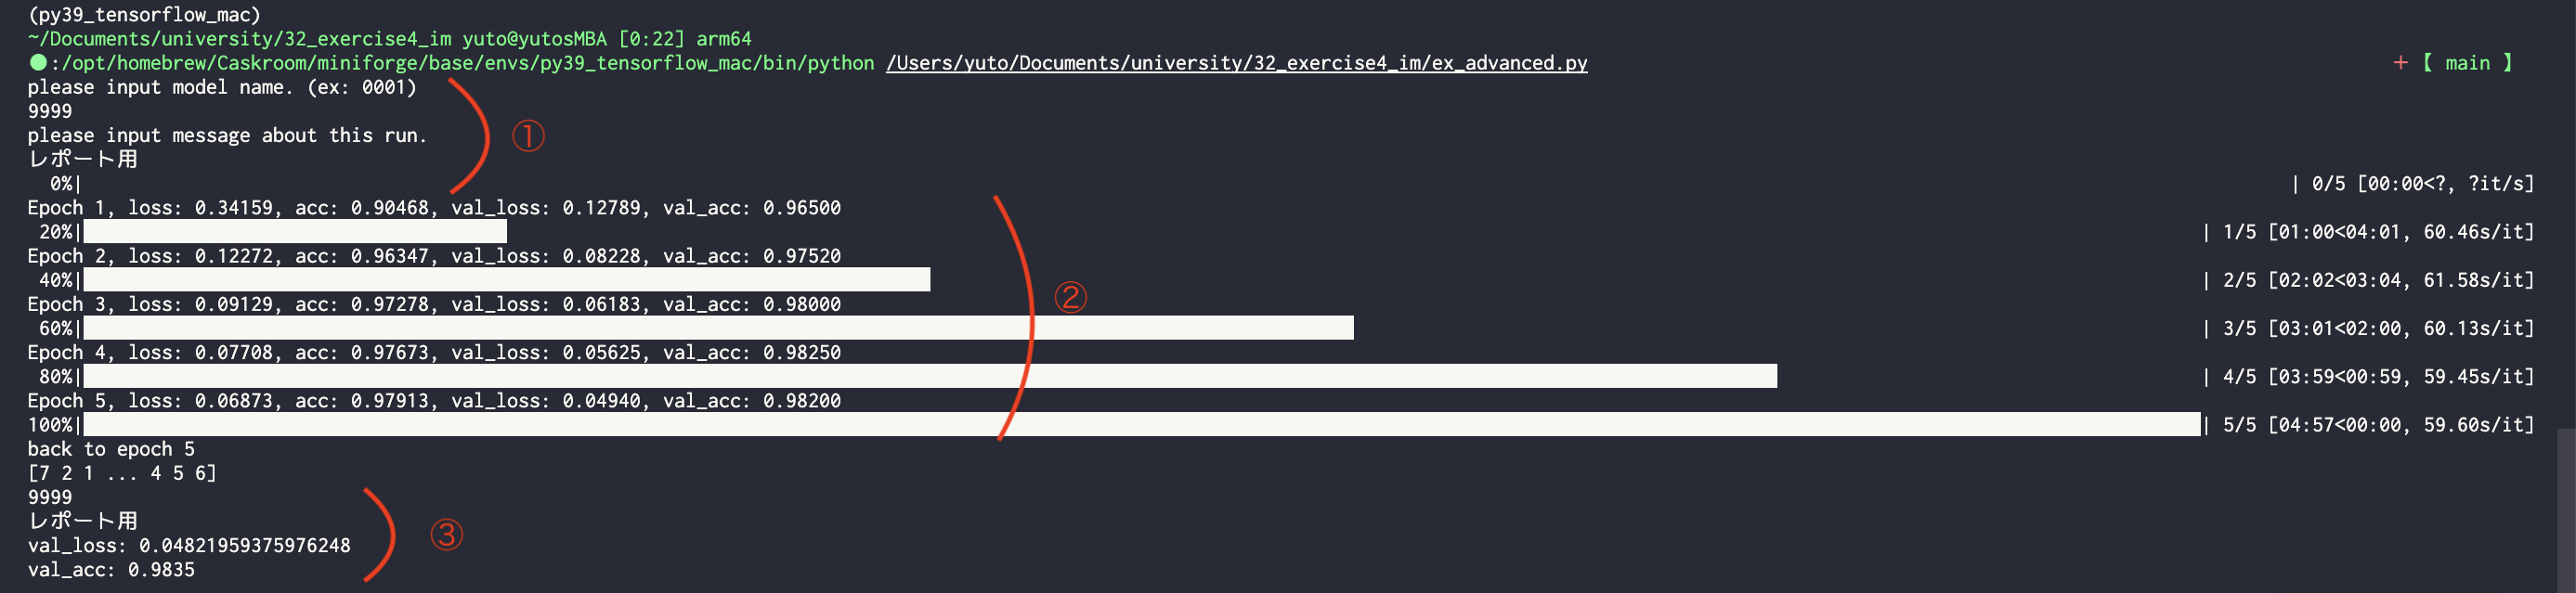
\includegraphics[width=15cm]{ex4_output.png}

\begin{quote}
\begin{verbatim}

1 : 実行の名前とメッセージを入力
2 : 学習時の損失と精度とプログレスバーを表示
3 : ログ出力
\end{verbatim}
\end{quote}

\subsection{プロット}

実行を終えると、エポック毎の損失と誤差のグラフを表示する。滑らかに描画するために、サイズ2の移動平均を使っている。

\begin{lstlisting}[caption=ex\_advanced.py]
  figure = plt.figure()
  plt.plot(history['loss'], label='loss')
  if 'val_loss' in history:
    plt.plot(moving_average_curve(history['val_loss'], 2), label='val_loss')
  plt.legend()
  plt.ylim((0, 0.15))
  plt.show()
  
  figure = plt.figure()
  plt.plot(history['acc'], label='acc')
  if 'val_acc' in history:
    plt.plot(moving_average_curve(history['val_acc'], 2), label='val_acc')
  plt.legend()
  plt.ylim((0.97, 1))
  plt.show()
\end{lstlisting}

なお、学習後に損失と重みをpickleで保存しているので後からグラフの表示も可能である。plot.ipynbに実装している。損失のグラフの実例を示す。

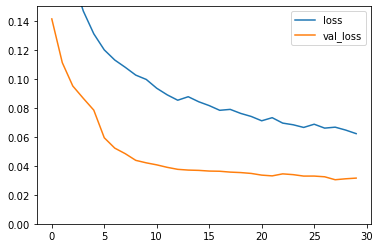
\includegraphics[width=10cm]{loss.png}

精度のグラフの実例を示す。

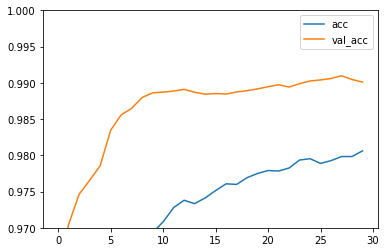
\includegraphics[width=10cm]{acc.png}

\newpage

\section{実験}

比較実験は様々行なったが、得られた主要なポイントを示す。

\begin{itemize}
  \item 畳み込み層は非常に大きく精度を向上させる。
  \item ネットワークの構造を大きくすると、MNIST程度のタスクだとすぐに過学習してしまう。
  \item 重みの初期値が大きいと、活性化関数でオーバーフローが起きやすい。
  \item ドロップアウトは過学習を抑制する。
  \item バッチノーマリゼーションとドロップアウトを同時に用いることは、必ずしも精度向上に寄与しない。
  \item プーリング層は必ずしも精度向上に寄与しない。
  \item 画像の正規化によって、活性化関数でオーバーフローが起きにくくなる
  \item Adamの方が高い精度を出すこともあれば、SGDと変わらないこともある。Adamは局所解を防ぐので、重みの初期値の影響を受けにくいからだと考えた。逆に言えば、初期値をうまく設定すれば、SGDも良い精度を出す。
\end{itemize}

実験の結果、検証データに対して単独で最も高い精度を出したモデルを示す。このモデルは、損失0.03201、
精度0.99を記録した。

\begin{table}[H]
  \begin{tabular}{lll}
    \hline
    Layer & Output & Parameter \\
    \hline \hline
    Input & (BS, 28, 28) & output\_shape=(28, 28) \\
    \hline
    Conv & (BS, 32, 28, 28) & input\_shape=(28, 28), filter\_shape=(5, 5), \\
    & & filter\_num=32, opt='Adam', opt\_kwds=\{\} \\
    \hline
    ReLU & (BS, 32, 28, 28)  \\
    \hline
    Pooling & (BS, 32, 14, 14) & input\_shape=(28, 28), channel=32, pool\_shape=(2, 2) \\
    \hline
    Flatten & (BS, 6272(=32*14*14)) \\
    \hline
    Dropout & (BS, 6272) & dropout=0.4 \\
    \hline
    Dense & (BS, 10) & units=10, input\_size=32*14*14, \\
    & & opt='Adam', opt\_kwds=\{\} \\
    \hline
    Softmax & (BS, 10) \\
    \hline
  \end{tabular}
\end{table}

\section{コンテスト}

学習データや検証データで良い精度を出すモデルであっても、コンテストのデータではあまり精度が出ない。これはコンテストのデータは学習データから特徴を捉えきれない、要は難しいデータであるからだと考えられる。そこで戦術として、

\begin{enumerate}
  \item モデルの構造とパラメータをチューニングして可能な限りスコアを高める
  \item データ拡張
  \item アンサンブル
\end{enumerate}

を用いて、特徴の取りこぼしを防ぐ。データ拡張は平行移動のみを用いた。アンサンブルについてはルールが曖昧だったが、アンサンブルによる精度向上が$1.9\%$であったことをここに記しておく。

\section{工夫点}

工夫点は数多くあるので、プログラムとともに詳細を説明してきた。特に力を入れて工夫したのが、コンテストに向けて比較実験を行いやすいように、モデルの拡張性、可変性を高めた点と、学習時の損失、精度の保存と、ログの出力である。

\section{問題点}

やれるだけのことをやり切った自信はあるが、強いて言うならば、データ拡張の種類をもう少し増やすことはできたかもしれない。

\section{添付について}
ディレクトリ構造を工夫したことを含めて見ていただきたいので、本実験のディレクトリごと添付した。主となるファイルはex\_advanced.py logger.py, plot.ipynb である。

\section{感想}

非常に楽しく、また勉強になりました。データ分析に興味があって、KerasやPyTorchを使っているものの、ニューラルネットの仕組みをきちんと理解できたのは、この実験のおかげです。畳み込みでうまくテンソル演算を組み合わせてfor分を減らすために、im2colとcol2imが編み出されたことには感動しました。コンテスト暫定1位も非常にうれしく思っています。

\end{document}
